\documentclass[12pt]{article}

\usepackage[T2A]{fontenc}
\usepackage[utf8x]{inputenc}
\usepackage[english, russian]{babel}
\usepackage{geometry}
\geometry{a4paper, portrait, margin=0.75in}
\usepackage{setspace}
\usepackage{graphicx}
\usepackage[normalem]{ulem}
\usepackage{float}

\begin{document}
\begin{titlepage}
    \begingroup
\fontsize{12pt}{14pt}\selectfont

\begin{center}

    Санкт-Петербургский политехнический университет имени Петра великого\\
    Институт компьютерных наук и кибербезопасности\\
    Высшая школа компьютерных технологий и информационных систем\\

    \vspace{\fill}

    \onehalfspacing
    \textbf{\huge Лабораторная работа \textnumero 12}\\
    \medbreak
    Дисциплина:\textbf{ Телекоммуникационные технологии}\\
    Тема: \textbf{ Пример моделирования BPSK демодуляции }\\
    \vspace{2.0cm}
\end{center}


\begin{flushright}
    \doublespacing
    Выполнил студент гр. 5130901{\textbackslash}10202 \underline{\hspace{7em}} Никаноренков М.Д.\\
    \smallskip
    Принял преподаватель \uline{\hspace{7em}}Богач Н.В. \\
    \smallskip
    "\uline{\hspace{1.5em}}" \uline{\hspace{5em}} 2024 г.\\
\end{flushright}

\vspace{\fill}

\begin{center}
    Санкт-Петербург\\
    2024 г.\\
\end{center}

\singlespacing

\pagebreak

\endgroup

\end{titlepage}

\tableofcontents
\pagebreak

\section{Постановка задачи:}

Изучить предложенную статью и пример моделирования BPSK демодуляции. Данная статья является продолжением QPSK\_Mod\_and\_Demod руководства, в котором описывается и использование BPSK. 

\section{Ход работы. Передача сигнала:}

Сначала необходимо пояснить, что разница между QPSK и BPSK заключается в количестве битов на символ. В QPSK используются 2-битные символы; в BPSK – 1-битные. В обоих случаях блок модулятора Constellation использует все 8 входных битов. Обратим внимание на то, что объект Constellation отличается в QPSK и BPSK.

Первый этап работы устройства – передача сигнала BPSK. 

Для этого генерируем поток битов и модулируем его в сложную совокупность с помощью блока модулятора Constellation. 

Объект constellation позволяет нам определить, как кодируются символы. Модулятор constellation ожидает упакованные байты, поэтому у нас есть генератор случайного источника, предоставляющий байты со значениями 0-255.

При работе с количеством выборок на символ мы хотим сохранить их минимальное значение ¬– здесь 2. Это значение можно использовать, чтобы согласовать желаемую скорость передачи данных с частотой дискретизации используемого аппаратного устройства. 

Поскольку в работе используется моделирование, выборки для каждого символа важны только для обеспечения соответствия скорости на всей потоковой диаграмме. Для моделирования возьмём значение 4, что больше, чем нам нужно, но полезно для визуализации сигнала в разных доменах.

Следующий этап – установка значения избыточной полосы пропускания. 

Модулятор constellation использует фильтр формирования импульсов с повышенным косинусом (RRC), который предоставляет единственный параметр для настройки коэффициента спада фильтра --- "альфа". 

Ниже представлена блок-схема bpsk\_stage1.grc: (См. Рис.1)

\begin{figure}[h]
    \centering
    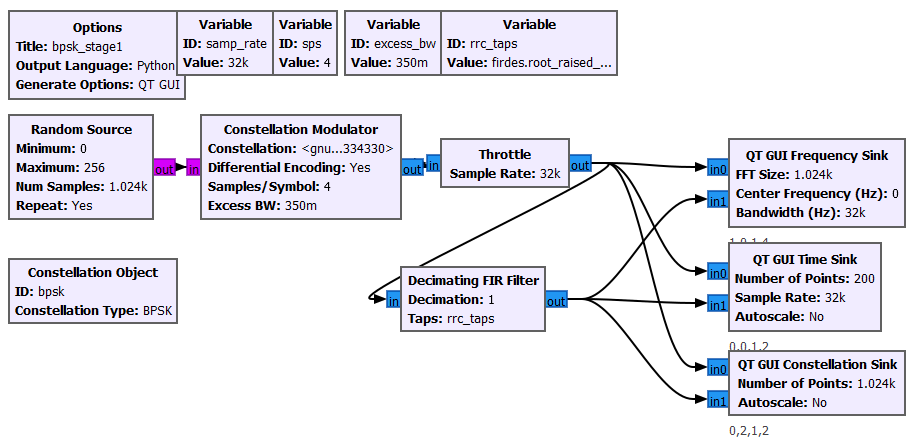
\includegraphics[width=1\textwidth]{pics/a0000-img001.png}
    \caption{Исследуемая блок-схема}
\end{figure}

\bigskip

Опишем основные блоки, использованные на данной схеме:

\begin{itemize}
	\item \textbf{Options} --- определяет имя файла для потоковой диаграммы, автора и т.д.
	\item \textbf{Random Source} --- cлучайный источник, генерирующий байтовые значения от 0 до 255.
	\item \textbf{Constellation Modulator} --- иерархический блок для дифференциальной универсальной модуляции с RRC-фильтрацией. Входным сигналом является поток байтов, а выходным - комплексно модулированный сигнал в основной полосе частот.
	\item \textbf{Throttle} --- ограничитель скорости передачи данных.
	\item \textbf{Decimating FIR Filter} --- "обычный" FIR-фильтр GNU Radio.
	\item \textbf{QT GUI Frequency Sink} --- графический приемник на основе QT, который принимает набор сложных потоков и используется для определения правильной центральной частоты.
	\item \textbf{QT GUI Time Sink} --- графический приемник, основанный на библиотеке QT, предназначенный для отображения нескольких сигналов во временной области.
	\item \textbf{QT GUI Constellation Sink} --- графический приемник для отображения созвездия IQ из нескольких сигналов.
	\item \textbf{Constellation Object} 
	\item \textbf{Variables} 
\end{itemize}

\textbf{Принцип работы передатчика:}
\begin{enumerate}
	\item Случайный источник генерирует байтовые значения от 0 до 255.
	\item При распаковке K битов каждый бит входных данных преобразуется в отдельный байт со значением в младшем значащем бите. 
	\item Поскольку аппаратное обеспечение не задействовано, для ограничения потока через систему используется блок Trottle.
\end{enumerate}

На графике (См. Рис.2, 3) мы видим эффекты увеличения выборки (генерация 4 выборок на символ) и процесса фильтрации. 

Фильтр RRC же добавляет преднамеренные собственные помехи, известные как межсимвольные помехи (ISI). ISI вреден для принимаемого сигнала, потому что он размывает символы вместе. 

Теперь посмотрим, как изменяется сигнал после воздействий на него. Сам по себе частотный график показывает сигнал с нормальной формой, который переходит в шум. Но если бы мы не наложили формирующий фильтр на сигнал, то передавали бы прямоугольные волны, которые производят много энергии в соседних каналах. 

За счет уменьшения внеполосных излучений наш сигнал теперь остается в пределах полосы пропускания нашего канала.

\begin{figure}[H]
    \centering
    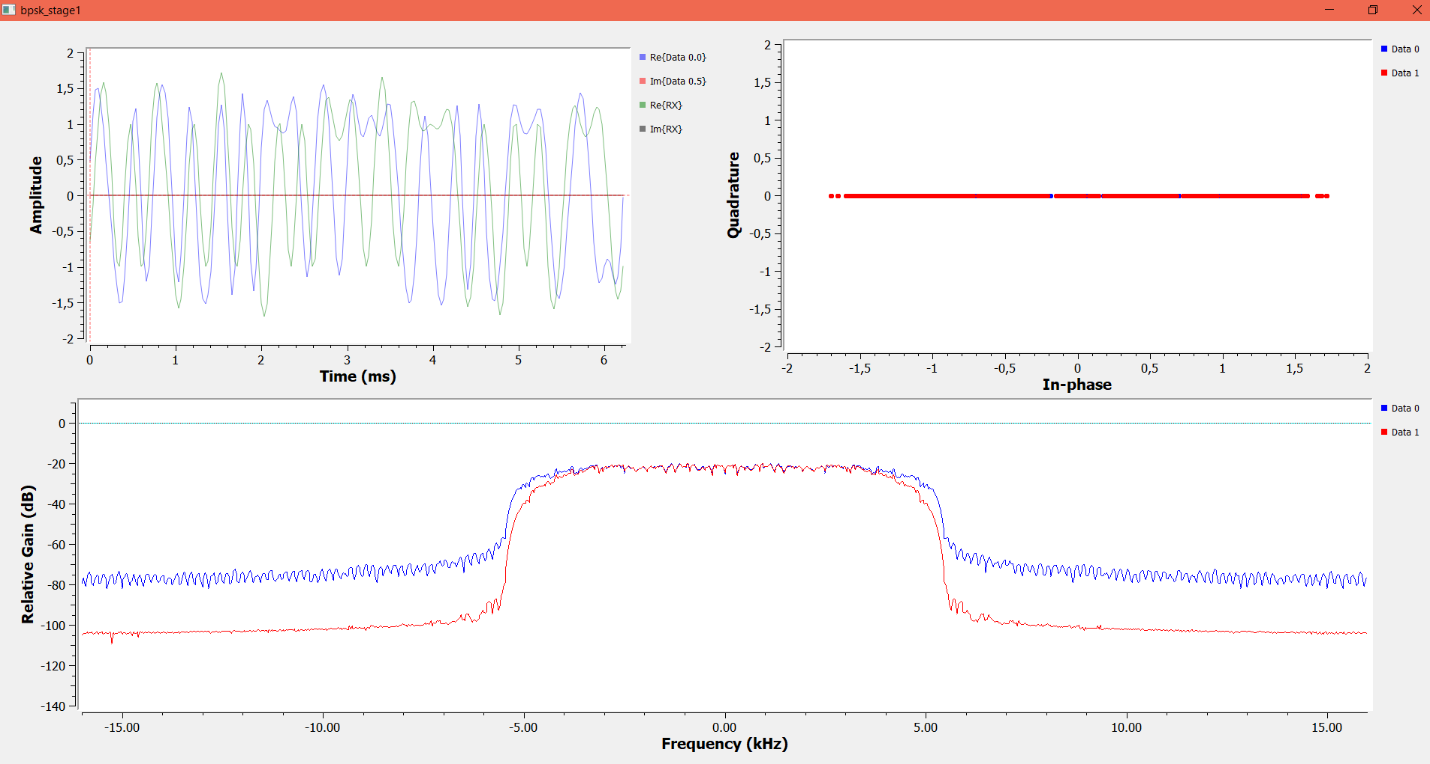
\includegraphics[width=1\textwidth]{pics/a0000-img002.png}
    \caption{Графики моделирования работы блок-схемы (1)}
\end{figure}

\begin{figure}[H]
    \centering
    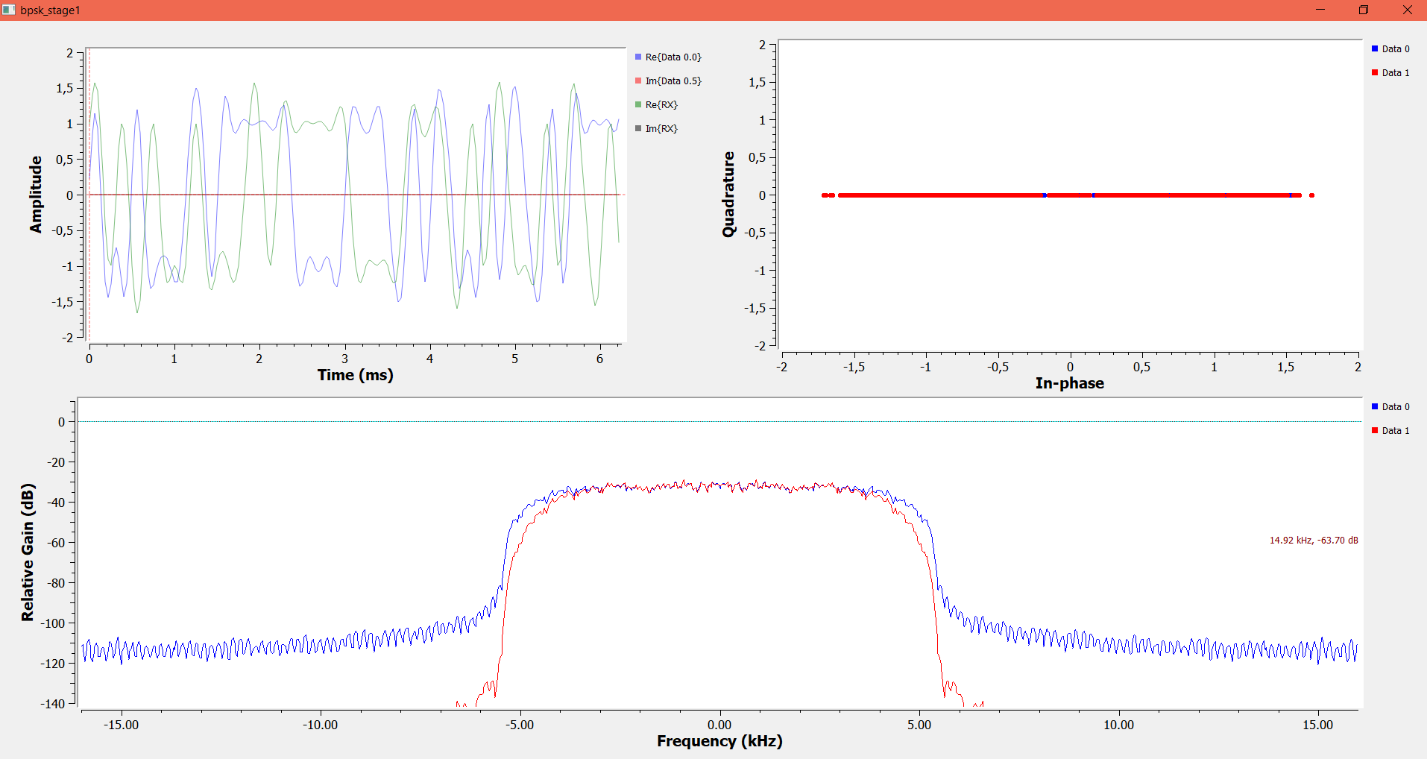
\includegraphics[width=1\textwidth]{pics/a0000-img003.png}
    \caption{Графики моделирования работы блок-схемы (2)}
\end{figure}

Далее, на стороне приема мы избавляемся от ISI, используя другой фильтр RRC. По сути, мы использовали фильтр на передатчике, RRC-фильтр, который создает ISI, но управляет полосой пропускания, а затем другой RRC-фильтр на приемнике. Таким образом, когда мы объединяем два RRC-фильтра, мы получаем фильтр повышенных косинусов. Выходной сигнал RRC-фильтра на стороне приема представляет собой сигнал в форме повышенного косинуса с минимизированным ISI.

\section{Добавление искажений канала:}

Теперь мы рассмотрим эффекты канала и то, как искажается сигнал в промежутке между моментом его передачи и моментом, когда мы видим сигнал в приемнике. 

Для этого добавим модель канала в блок-схему, представленную выше. В работе мы используем базовый блок модели канала GNU Radio: 

\begin{figure}[H]
    \centering
    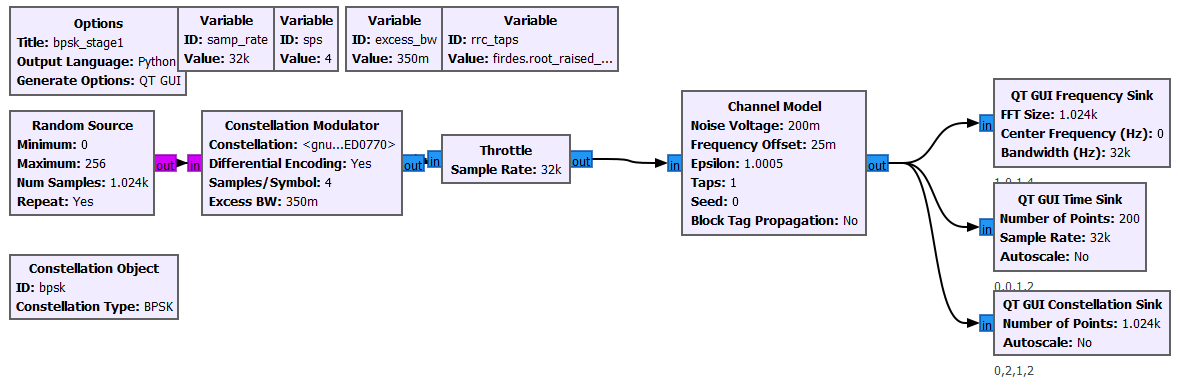
\includegraphics[width=1\textwidth]{pics/a0000-img004.png}
    \caption{Блок-схема с моделью канала}
\end{figure}

Блок Channel Model позволяет смоделировать несколько основных проблем, с которыми нам приходится иметь дело:

\begin{enumerate}
	\item Шум. Тепловой шум в приемнике вызывает шум, который мы знаем как аддитивный белый гауссовский шум (AWGN). Теперь мы сами устанавливаем мощность шума, регулируя значение напряжения шума модели канала. 
	\item Разные часы, которые определяют частоту радиостанций. Часы, во-первых, несовершенны, и поэтому разные радиостанции различаются. Восстановление синхронизации
\end{enumerate}

Результат моделирования представлен на Рис.5:

\begin{figure}[H]
    \centering
    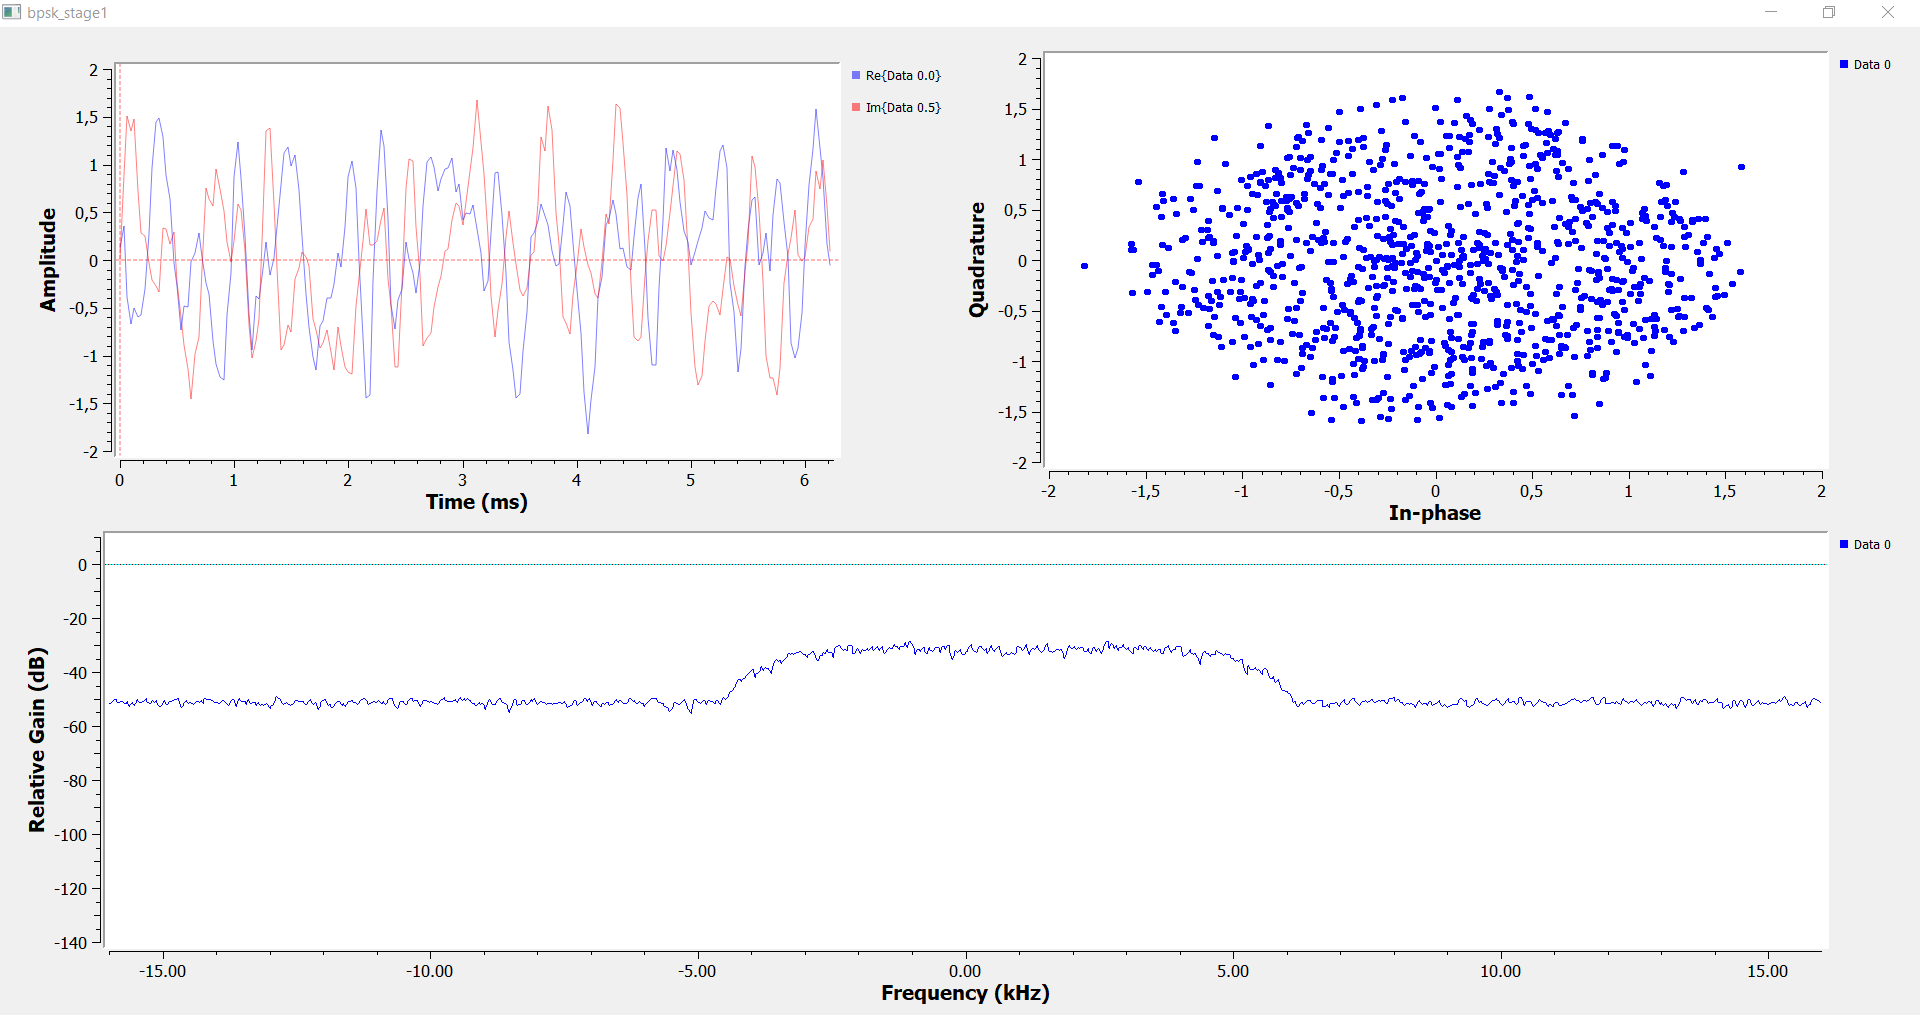
\includegraphics[width=1\textwidth]{pics/a0000-img005.png}
    \caption{Диаграммы работы блок-схемы с моделью канала}
\end{figure}

\section{Восстановление синхронизации:}

Многофазная синхронизация часов выполняет три функции. Во-первых, она выполняет восстановление синхронизации часов. Во-вторых, она предоставляет фильтр согласования с приемником для удаления ISI. В-третьих, он уменьшает дискретизацию сигнала (уменьшает количество выборок на символ).

Блок-схема Bpsk\_stage3.grc Представлена ниже:

\begin{figure}[H]
    \centering
    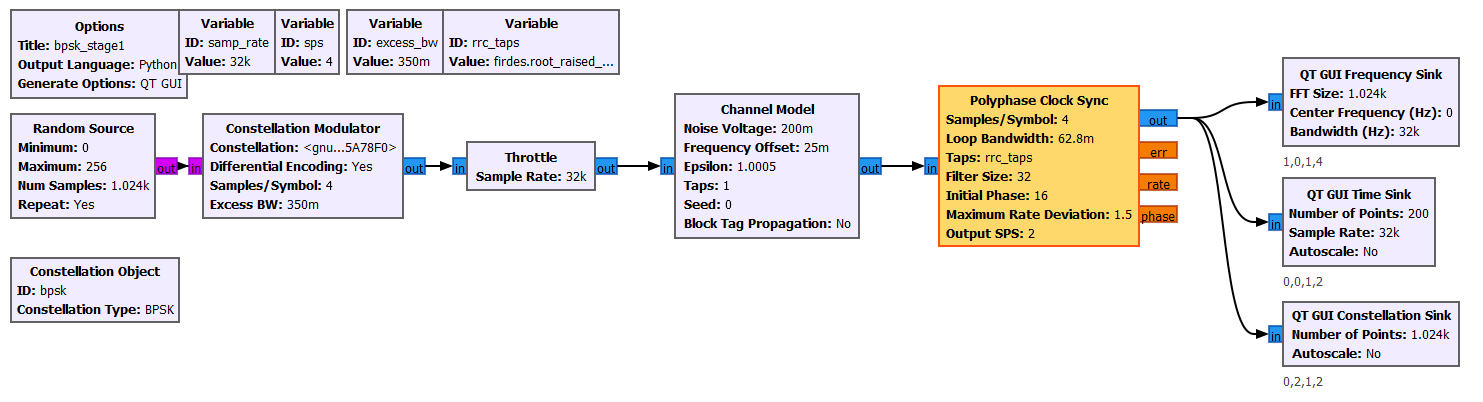
\includegraphics[width=1\textwidth]{pics/a0000-img006.png}
    \caption{Блок-схема с модулем синхронизации}
\end{figure}

Данная схема принимает выходные данные модели канала и передает их через блок многофазной синхронизации. Этот блок настроен с 32 фильтрами и пропускной способностью контура 2pi / 100. Блок также принимает значение ожидаемых выборок для каждого символа.

В результате моделирования (См. Рис.7) мы видим, что в созвездии все еще немного шумно из-за ISI после 32 фильтров, но оно быстро поглощается шумом, как только мы устанавливаем значение напряжения шума канала больше 0.

\begin{figure}[H]
    \centering
    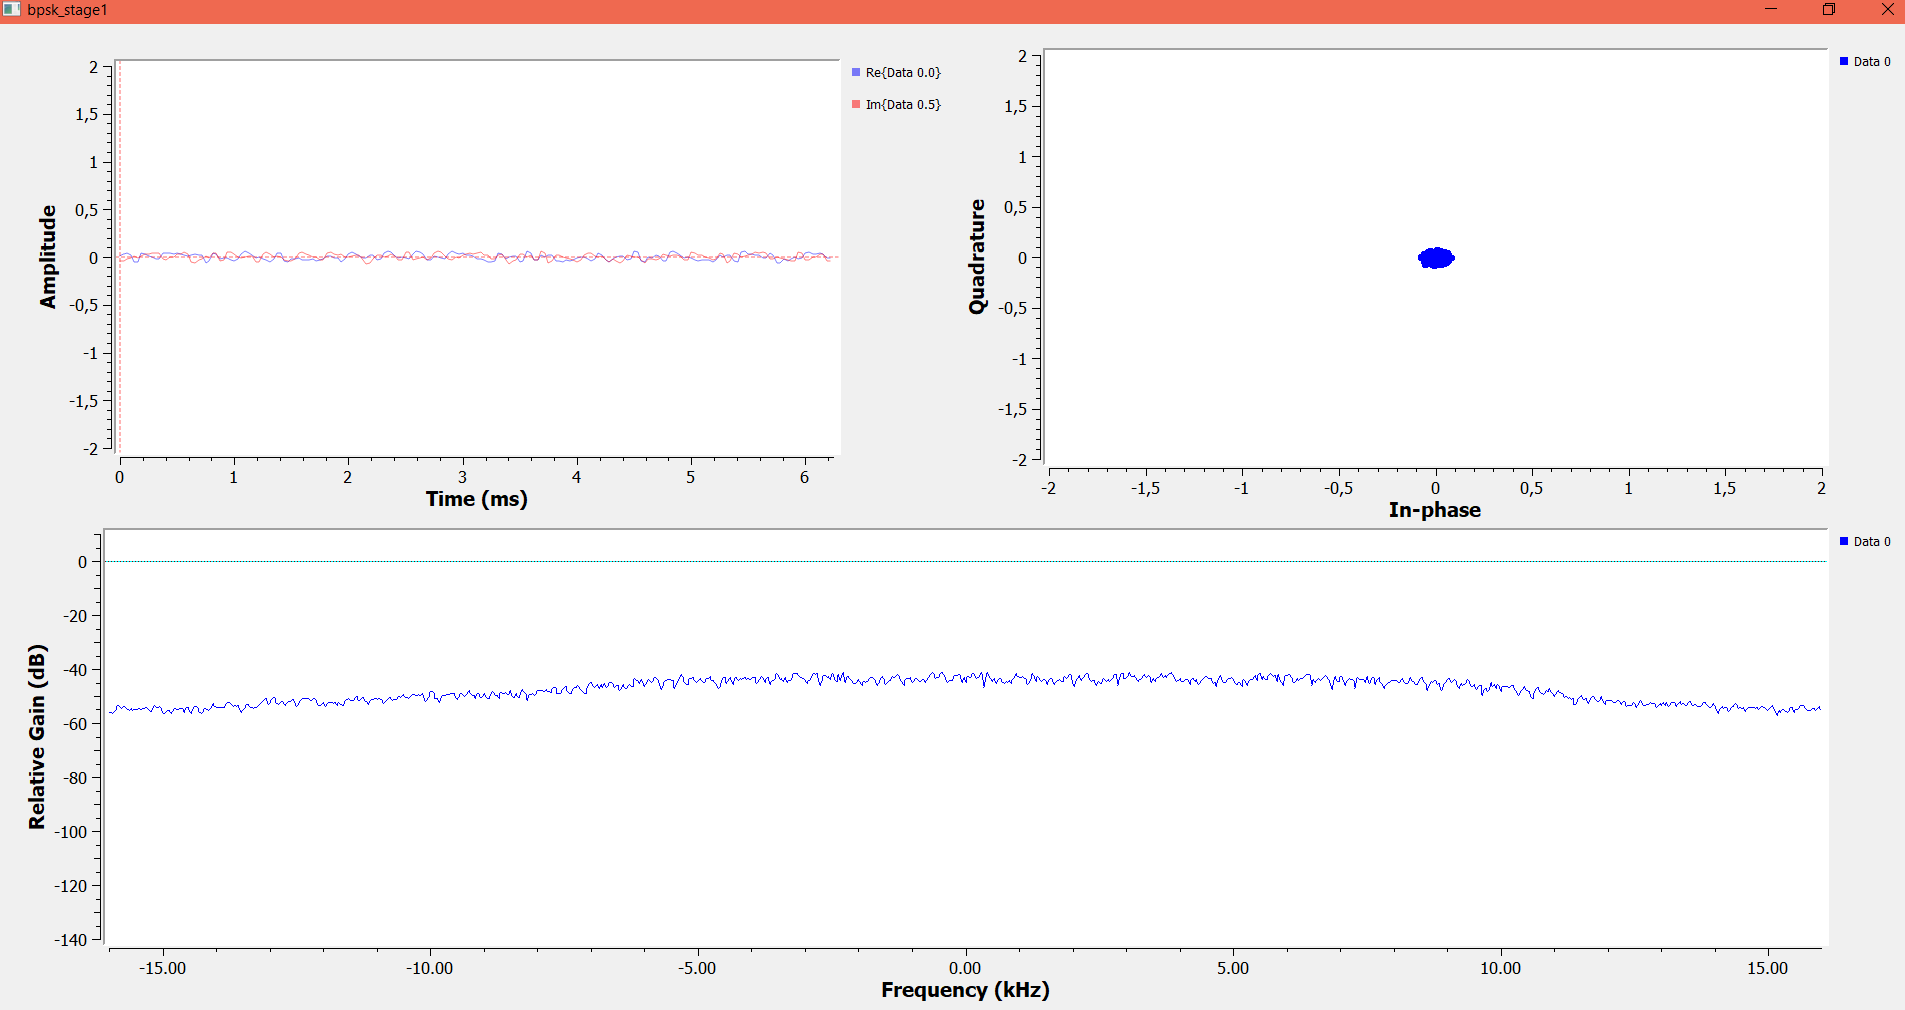
\includegraphics[width=1\textwidth]{pics/a0000-img007.png}
    \caption{Диаграммы работы блок-схемы с модулем синхронизации}
\end{figure}

\section{Фазовая и точная частотная коррекция:}

Учитывая, что мы выровняли канал, у нас все еще есть проблема со смещением фазы и частоты. Эквалайзеры, как правило, не адаптируются быстро, и поэтому простое смещение частоты может оказаться за пределами возможностей эквалайзера. Теперь нам нужно скорректировать любое смещение фазы, а также любое смещение частоты.

Две особенности этого этапа: 

\begin{itemize}
	\item Использование цикла второго порядка, чтобы мы могли отслеживать как фазу, так и частоту (которая является производной от фазы) с течением времени. 
	\item Тип восстановления, с которым мы здесь будем иметь дело, предполагает, что мы выполняем точную коррекцию частоты. Поэтому мы должны быть уверены, что мы уже находимся в приличном диапазоне идеальной частоты. 
\end{itemize}

Для этой задачи используем модуль Costas loop. Блок-схема для моделирования представлена на Рис.8: 

\begin{figure}[H]
    \centering
    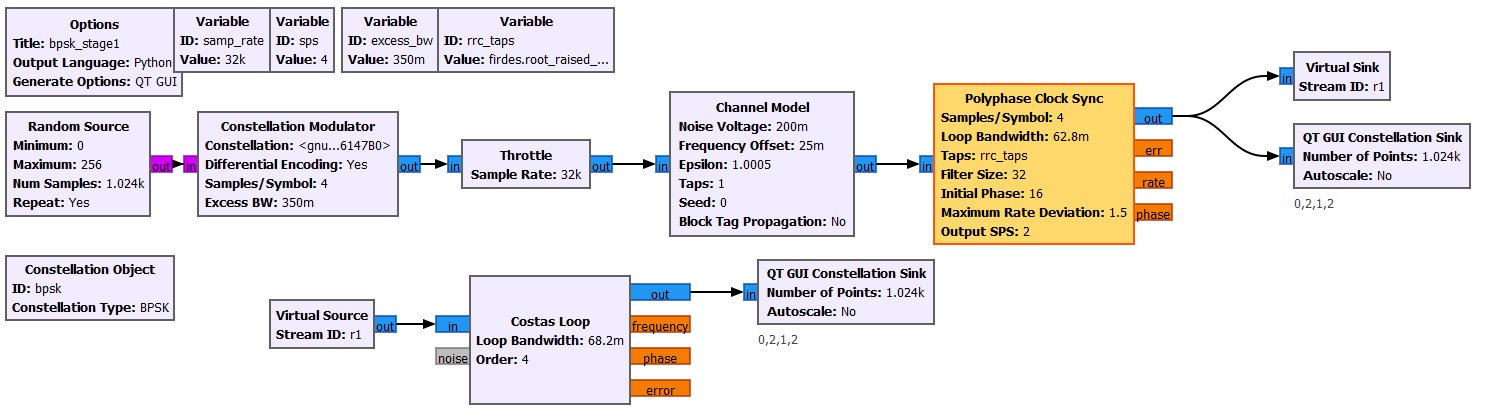
\includegraphics[width=1\textwidth]{pics/a0000-img008.png}
    \caption{Блок-схема с модулем Costas loop}
\end{figure}

Циклический блок Costas может синхронизировать BPSK, QPSK и 8PSK. Как и все другие наши модули, он использует цикл второго порядка и, следовательно, определяется параметром пропускной способности цикла. 

\pagebreak

Результат моделирования следующий:

\begin{figure}[H]
    \centering
    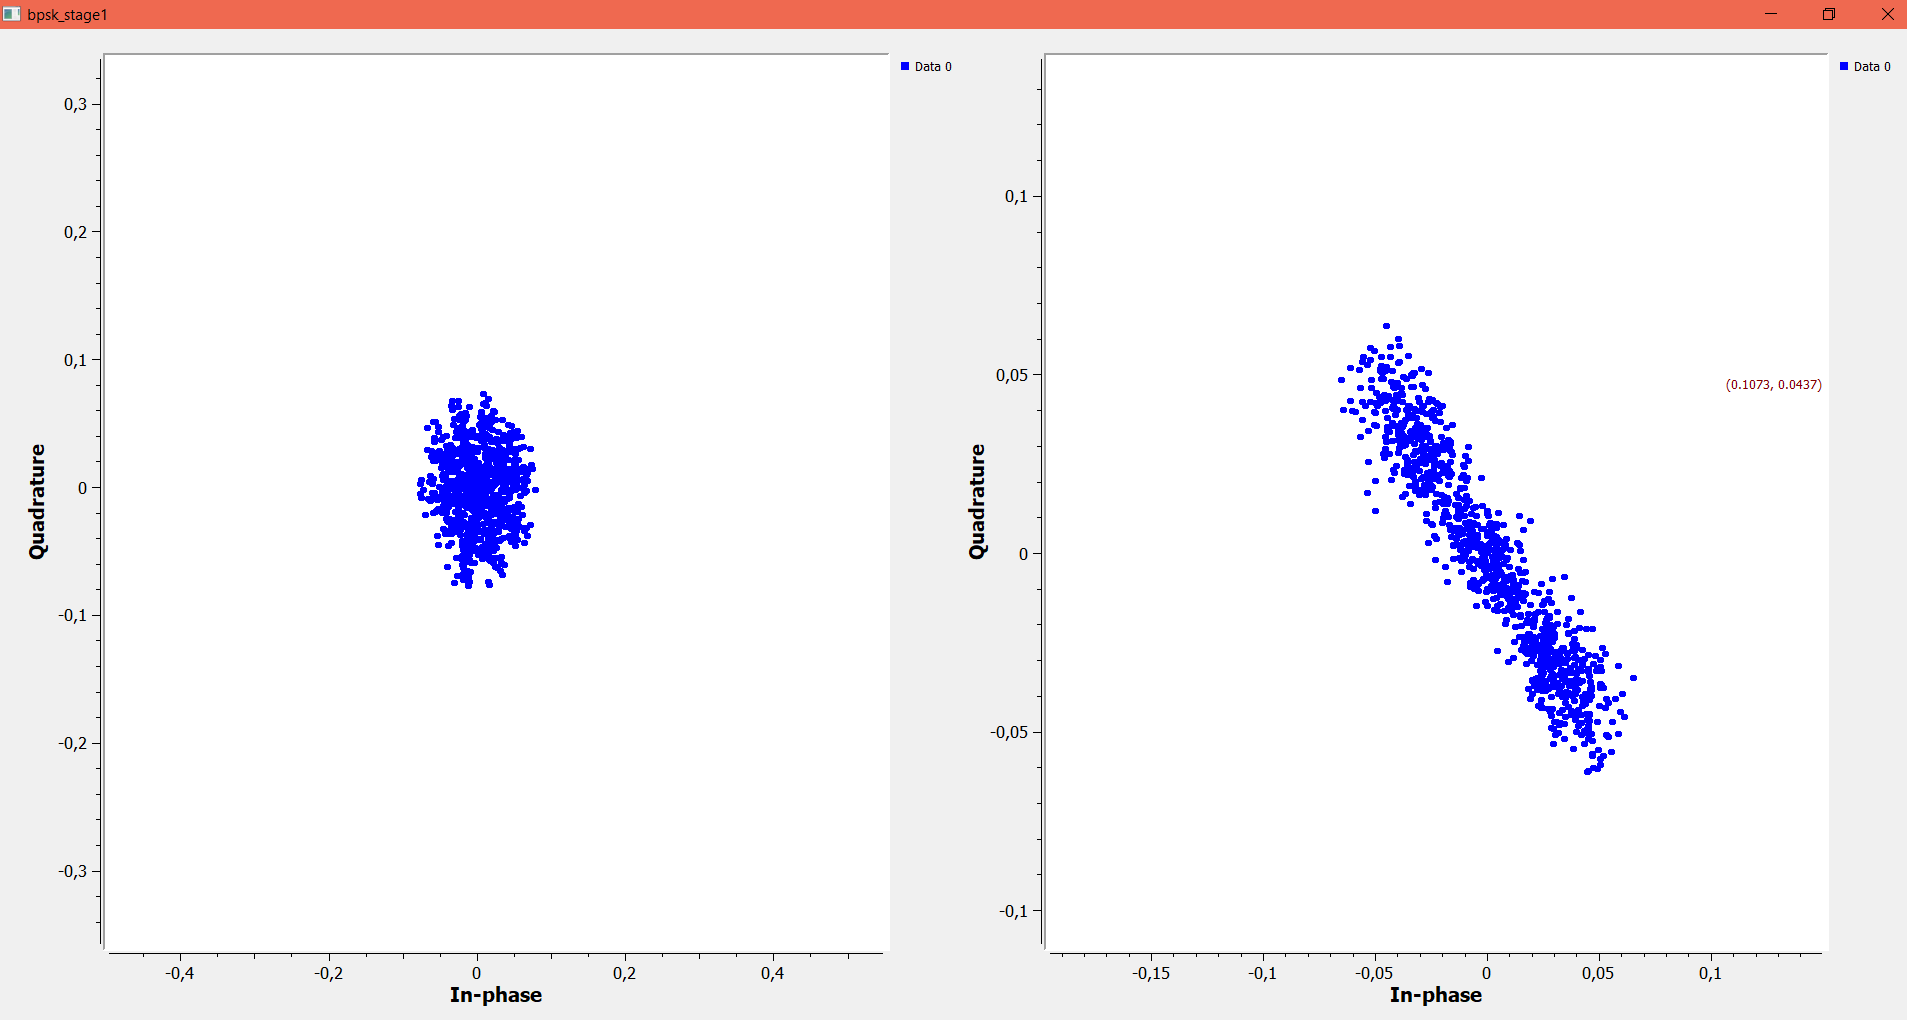
\includegraphics[width=1\textwidth]{pics/a0000-img009.png}
    \caption{Диаграммы работы блок-схемы с модулем Costas Loop}
\end{figure}


\section{Декодирование:}

Теперь, мы приступаем к декодированию сигнала. Блок-схема для завершающего этапа работы на Рис.10:

\begin{figure}[H]
    \centering
    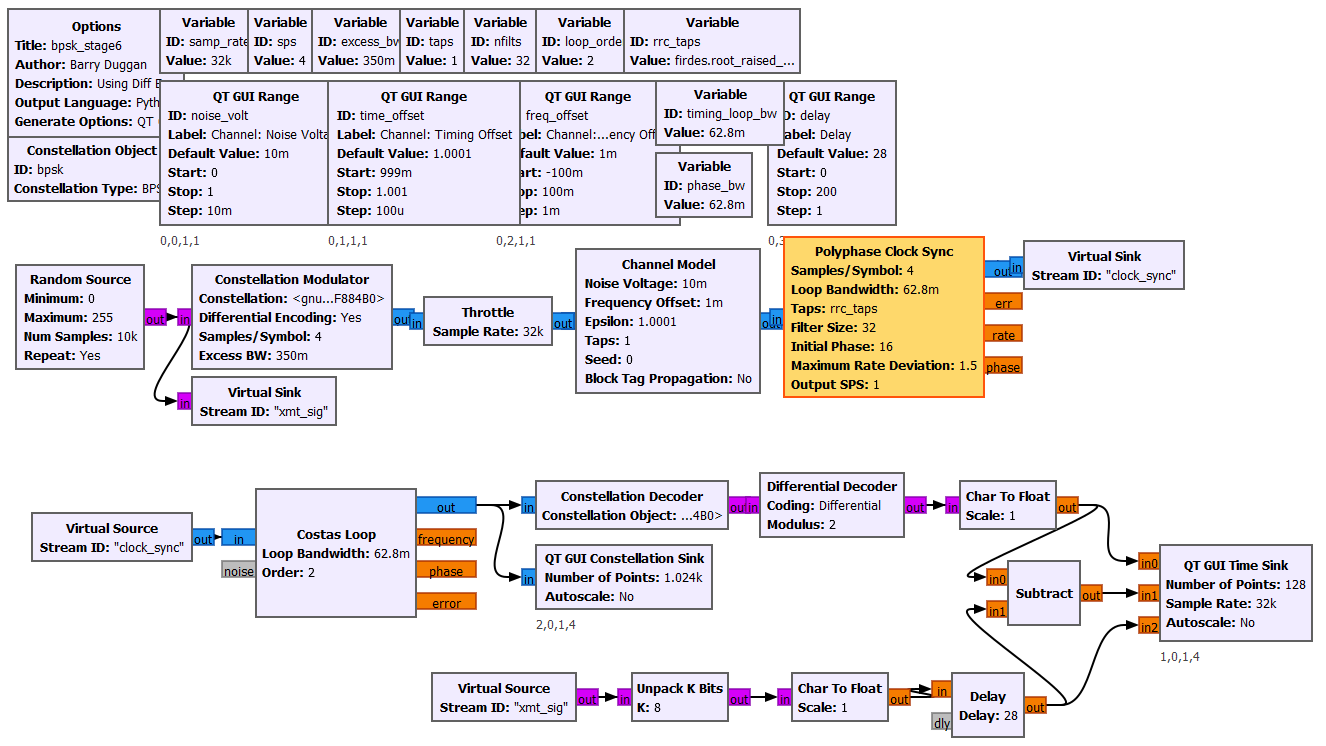
\includegraphics[width=0.8\textwidth]{pics/a0000-img010.png}
    \caption{Блок-схема с модулем декодирования}
\end{figure}

\pagebreak

На этом этапе мы получаем символы 0 и 1, потому что это размер алфавита в схеме BPSK. Но чтобы убедиться, что у нас такое же отображение символов на точки созвездия, которое мы использовали при передаче, вспомним про дифференциальные символы – на самом деле, мы не передавали само созвездие, мы передавали разницу между символами созвездия, установив дифференциальную настройку в блоке модулятора созвездия на "Yes". Итак, теперь мы это отменяем.

Блок-схема использует блок дифференциального декодера для преобразования дифференциально закодированных символов обратно в их исходные символы на основе фазовых переходов, а не самой абсолютной фазы. Теперь у нас есть исходный поток битов.

Убедимся в том, что перед нами исходный поток битов – сравним его с входным потоком. 

Прямое сравнение этих двух значений не показательно, поскольку цепочка приемников имеет множество блоков и фильтров, которые задерживают сигнал, поэтому принятый сигнал отстает на некоторое количество битов. Для компенсации задержим передаваемые биты на ту же величину, используя блок Delay. Как видно из Рис.6.3, подходящее значение задержки составило 25. Полученные диаграммы представлены на Рис.11, 12:

\begin{figure}[H]
    \centering
    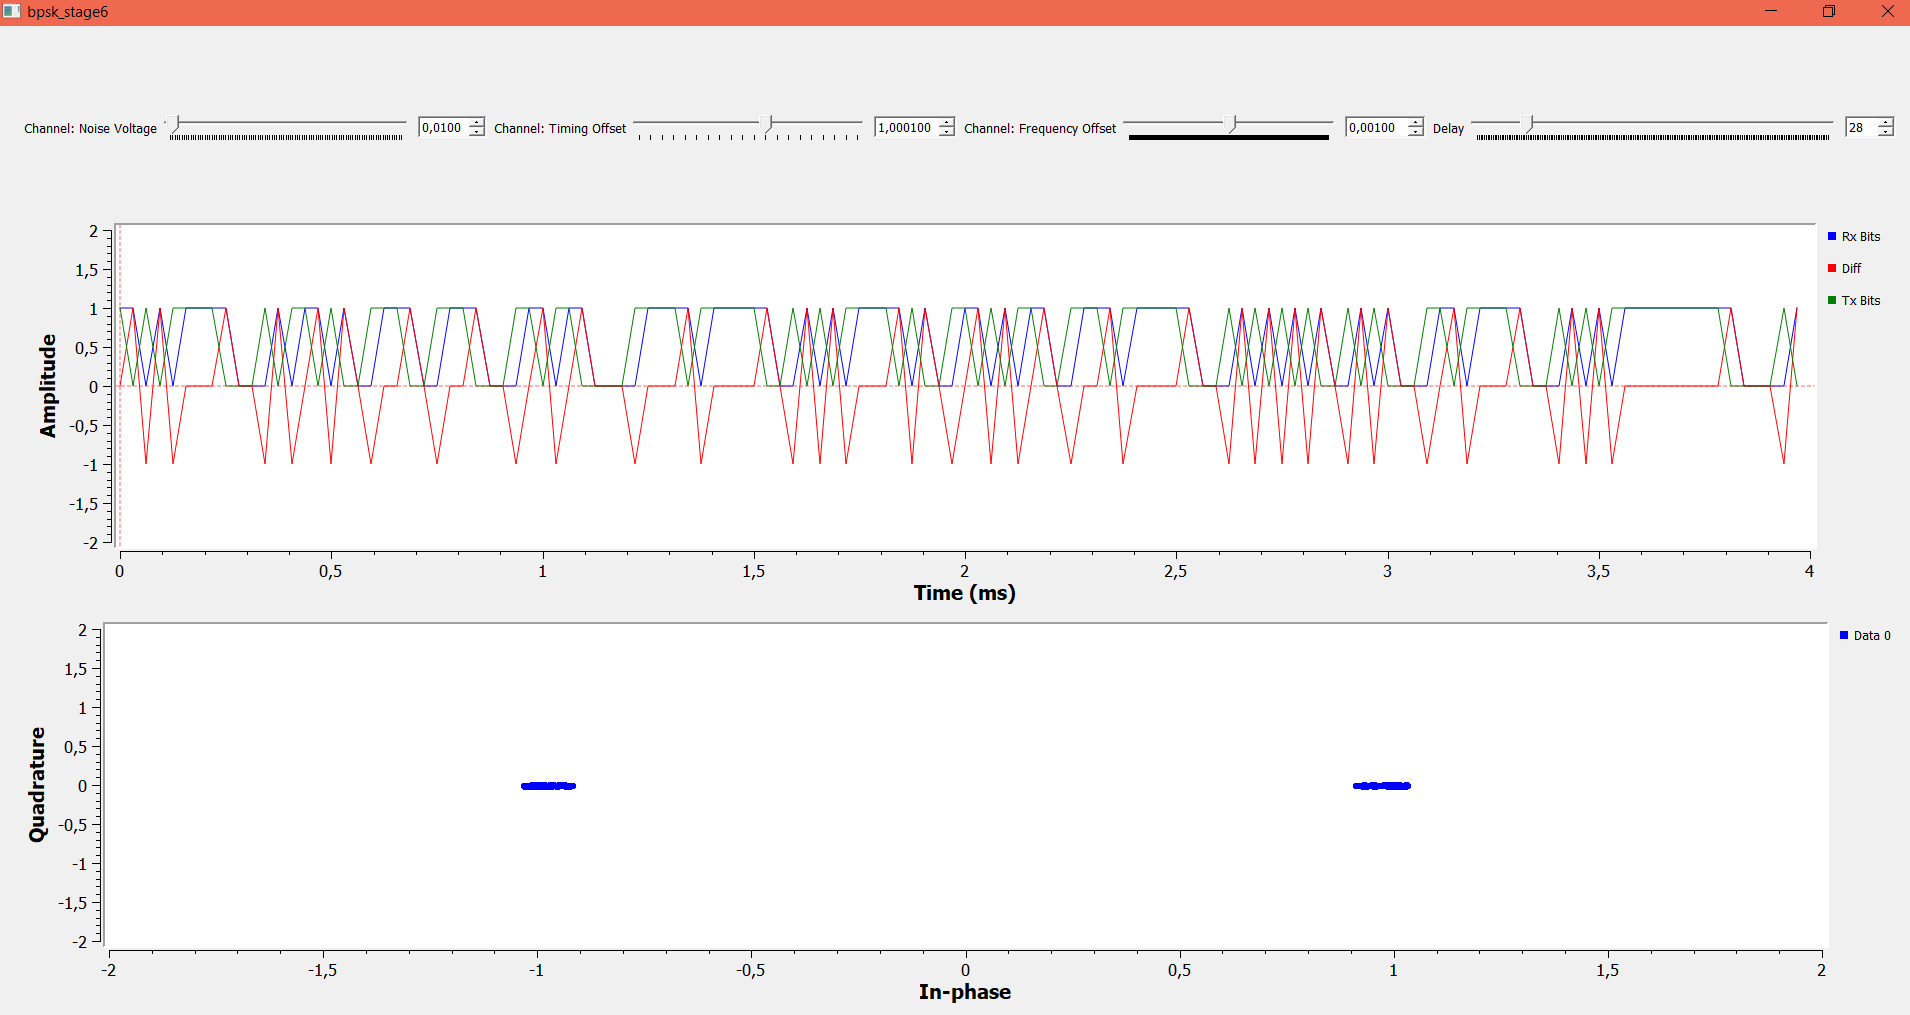
\includegraphics[width=0.75\textwidth]{pics/a0000-img011.png}
    \caption{Диаграммы работы итоговой блок-схемы без Delay}
\end{figure}

\begin{figure}[H]
    \centering
    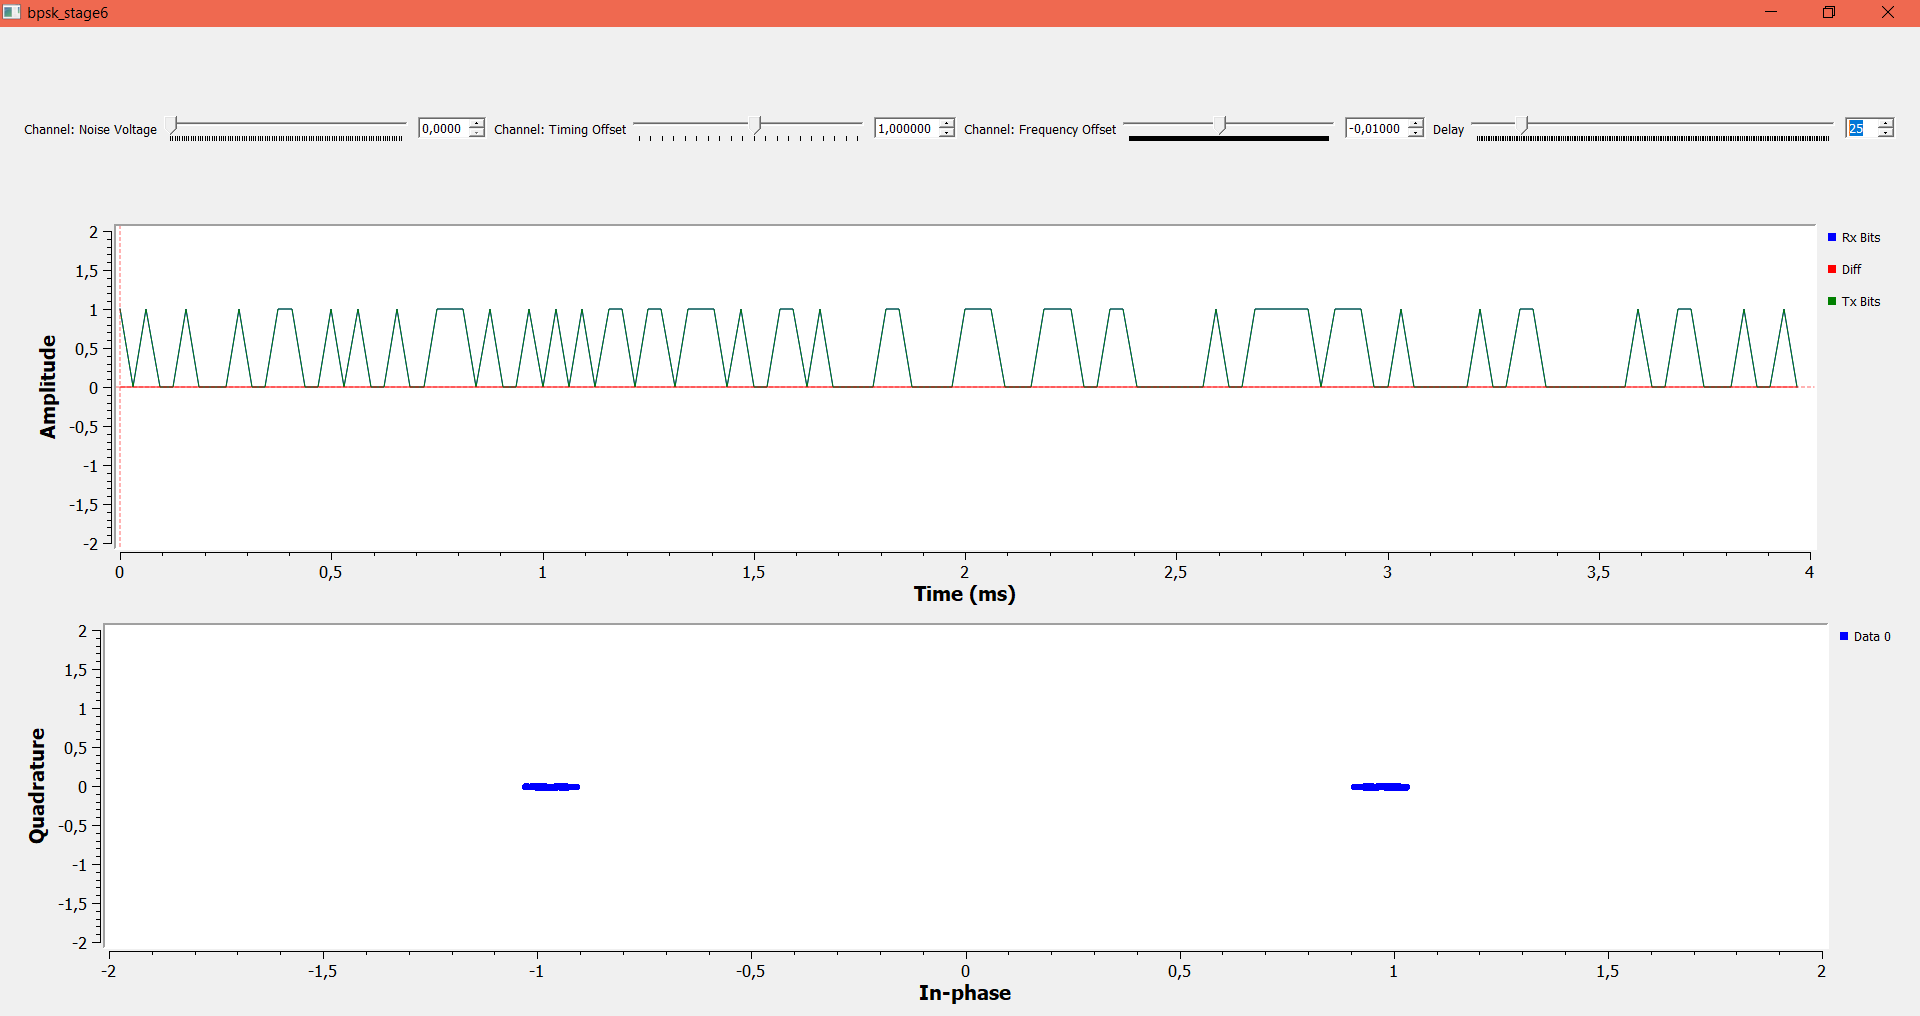
\includegraphics[width=0.75\textwidth]{pics/a0000-img012.png}
    \caption{Диаграммы работы итоговой блок-схемы с компенсацией задержки}
\end{figure}

Работа выполнена успешно.

\end{document}


